\documentclass{article}
\usepackage[utf8]{inputenc}
\usepackage{amsmath}
\usepackage{braket}
\usepackage{gensymb}
\usepackage{amssymb}
\usepackage{natbib}
\usepackage{graphicx}
\usepackage{listings}
\usepackage{color}
\usepackage{tikz}
\usepackage{multicol}
\usetikzlibrary{arrows}
\usepackage{float}
\restylefloat{figure}

\usepackage[figurename=Figure]{caption}

\definecolor{codegreen}{rgb}{0,0.6,0}
\definecolor{codegray}{rgb}{0.5,0.5,0.5}
\definecolor{codepurple}{rgb}{0.58,0,0.82}
\definecolor{backcolour}{rgb}{0.95,0.95,0.92}
 
\lstdefinestyle{mystyle}{
    backgroundcolor=\color{backcolour},   
    commentstyle=\color{codegreen},
    keywordstyle=\color{magenta},
    numberstyle=\tiny\color{codegray},
    stringstyle=\color{codepurple},
    basicstyle=\footnotesize,
    breakatwhitespace=false,         
    breaklines=true,                 
    captionpos=b,                    
    keepspaces=true,                 
    numbers=left,                    
    numbersep=5pt,                  
    showspaces=false,                
    showstringspaces=false,
    showtabs=false,                  
    tabsize=2
}
 
\lstset{style=mystyle}
\lstset{
    language=Erlang,
    mathescape=true
}
\usepackage{hyperref}
\hypersetup{
    colorlinks=true,
    linkcolor=blue,
    filecolor=magenta,      
    urlcolor=cyan,
}

\title{MEK1100 - Oblig 2}
\author{Hans-Petter Harveg}
\date{April 2018}

\begin{document}

\maketitle

\section*{Oppsummering}
Vi analyserer et dataset målt i Hydrodynamisk labratorium ved UiO. Vi gjør først noen tester på datasettet, deretter benytter vi nummeriske metoder for analyse av datasettet. Vi regner ut typiske størrelser og bruker Stokes, Greens sats og Gauss. Resultatene viser noe avvik, noe som er forventet når man tar høyde for nummeriske feil og unøyaktighet i målinger.

\section*{Besvarelse}

\subsection*{a$)$}

I denne oppgaven har jeg lastet inn datafilen og skrevet testfunksjoner for de gitte oppgavene. Spesifikt har jeg skrevet følgende funksjoner
\begin{itemize}
\item \textit{get\_matrix\_sizes()}: skriver ut dimensjonene på matrisen ved hjelp av funksjonen \textit{shate()}.
\item \textit{test\_pixel\_spread()}: sjekker at bredden mellom pixlene er 0.5. Fordi vi har en matrise med x-verider og en med y-verdier sjekker jeg begge matrisene. Funksjonen returnerer \textit{False} dersom den finner en verdi $\Delta x \neq 0.5$.
\item \textit{test\_y\_range()}: sjekker at dataen spenner høyden på røret.
\end{itemize}
Kjøreeksempelet ser ut som følger
\begin{lstlisting}
Size of [ yit ]: 194 1
Size of [ xit ]: 194 1
Size of [ v ]: 194 201
Size of [ y ]: 194 201
Size of [ x ]: 194 201
Size of [ u ]: 194 201

Grid is evenly spread, looks good!

Spread in y direction:
[[-50.  -50.  -50.  ..., -50.  -50.  -50. ]
 [-49.5 -49.5 -49.5 ..., -49.5 -49.5 -49.5]
 [-49.  -49.  -49.  ..., -49.  -49.  -49. ]
 ..., 
 [ 49.   49.   49.  ...,  49.   49.   49. ]
 [ 49.5  49.5  49.5 ...,  49.5  49.5  49.5]
 [ 50.   50.   50.  ...,  50.   50.   50. ]]
\end{lstlisting}
Koden i sin helhet ligger under \hyperlink{sourcecode}{kildekode}.

\subsection*{b$)$}
I denne oppgaven har jeg laget to plot
\begin{figure}[H]
\centering
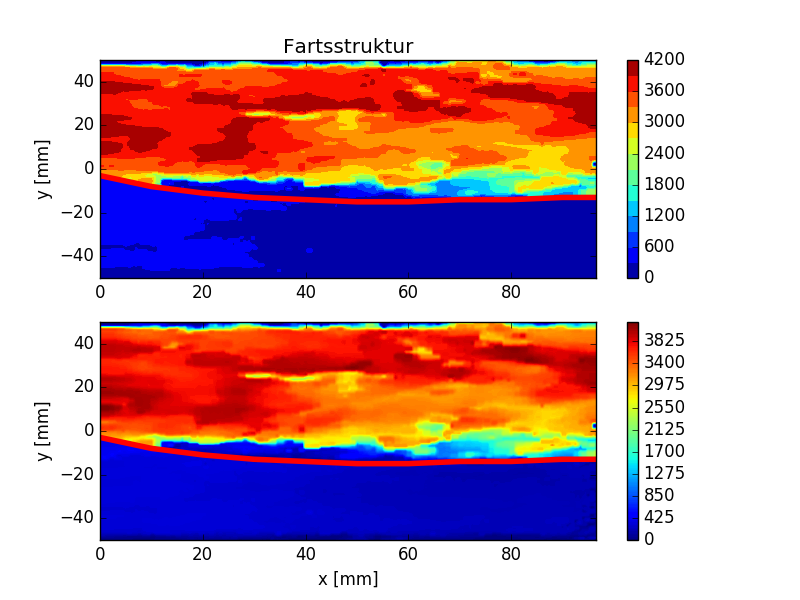
\includegraphics[width=0.6\textwidth]{problem_b}
\caption{Fartstruktur i vann og luft. Den rød linjen markerer skillet mellom vann og luft.}
\label{fig:problem_b_contour_fig}
\end{figure}


\subsection*{c$)$}
I denne oppgaven plotter jeg hastighetene ved hjelp av funksjonen \textit{quiver()}. Fordi antallet punkgter er høyt viser jeg kun hver 5. pil. Grunnen til at pilene vises som punkter er fordi forskjellden i hastighet her svært forskjellig i vann og luft.
\begin{figure}[H]
\centering
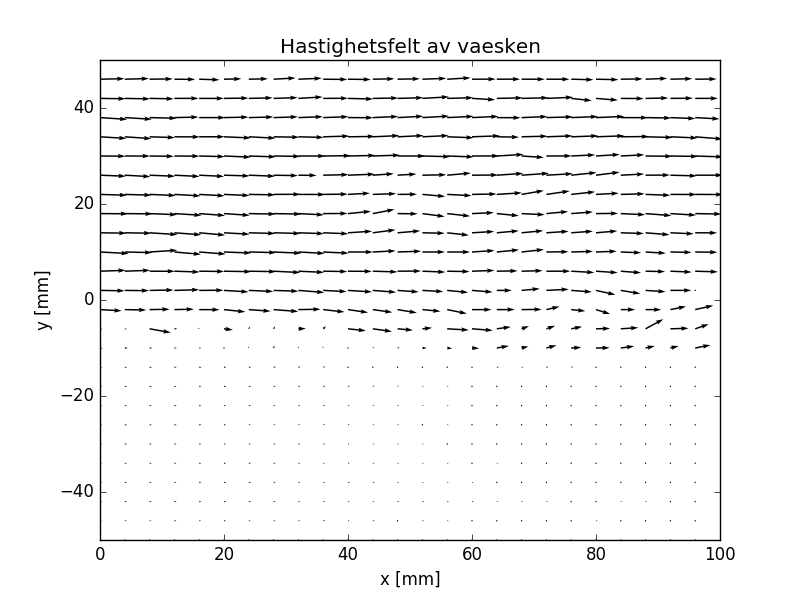
\includegraphics[width=0.6\textwidth]{problem_c_1}
\caption{Fordi hastigheten er så liten i vannet i forhold til i lufta er det vanskelig å se vektorpilene.}
\label{fig:problem_b_vector_fig}
\end{figure}
Ved å bruke indeksene gitt i oppgaven henter jeg ut koordinater fra datasettet. Disse bruker jeg til å plotte tre firkanter inn i figuren.
\begin{figure}[H]
\centering
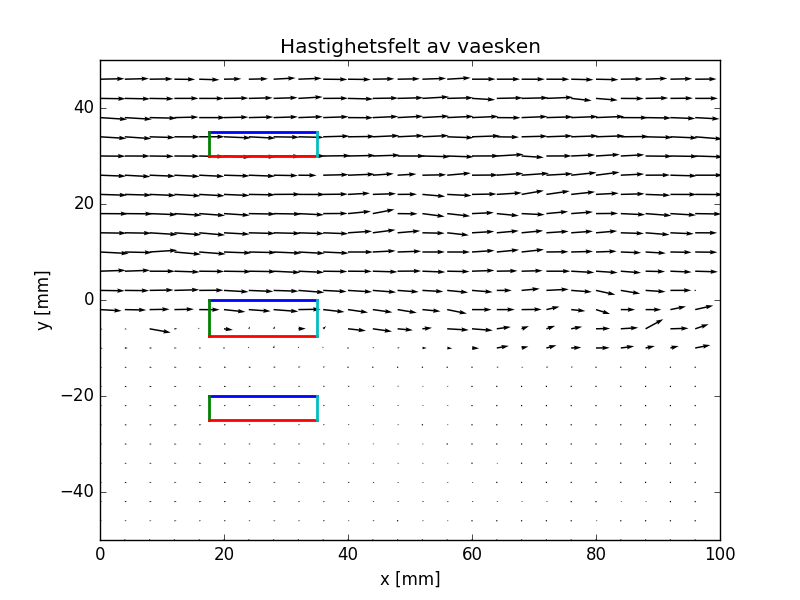
\includegraphics[width=0.6\textwidth]{problem_c_2}
\caption{Fordi hastigheten er så liten i vannet i forhold til i lufta er det vanskelig å se vektorpilene.}
\label{fig:problem_b_vector_fig}
\end{figure}


\subsection*{d$)$}
Divergensen til $\vec{v}$ er gitt ved
\begin{equation}
\nabla\cdot\vec{v} = \frac{\partial}{\partial x}u + \frac{\partial}{\partial y}v + \frac{\partial}{\partial z}w,
\end{equation}
men måten eksperimentet er satt opp på gir $\frac{\partial}{\partial z}w = 0$.
Imkompressibel vil si at når man følger en fluidpartikkel gjennom et hastighetsfelt vil den ha konstant tetthet
\begin{equation}
\frac{D\rho}{dt} = 0.
\end{equation}
Derav fra kontinuitetsligningen har vi at
\begin{equation}
\frac{D\rho}{dt} + \rho\nabla\cdot\vec{v} = 0,
\end{equation}
hvor vi har at $\nabla\cdot\vec{v} = 0$ for imkomprissibelt fluid. Dette betyr at $\nabla\cdot\vec{v} = 0$
\begin{equation}
\frac{\partial}{\partial z}w = -\bigg(\frac{\partial}{\partial x}u + \frac{\partial}{\partial y}v\bigg)
\end{equation}

\subsection*{e$)$}
Virvlingen til $\vec{v}$ er gitt ved
\begin{equation}
\nabla\cdot\vec{v} = \begin{vmatrix}\hat{i}&\hat{j}&\hat{k}\\\partial_{x}&\partial_{y}&\partial_{z}\\u&v&w\end{vmatrix}. 
\end{equation}
Som gir
\begin{equation}
\hat{k}\bigg(\frac{\partial}{\partial_{x}}v - \frac{\partial}{\partial_{y}}u \bigg),
\end{equation}
altså komponenten \textit{normalt på xy-planet}.
Hvis vi definerer ett nytt hastighetsfelt
\begin{equation}
\vec{v}' = v\hat{i} - u\hat{j},
\end{equation}
får vi at komponenten \textit{normalt på xy-planet} som
\begin{equation}
\hat{k}\bigg( \frac{\partial}{\partial x}v - \frac{\partial}{\partial y}u \bigg) = \hat{k}\nabla\cdot\hat{v}
\end{equation}


\subsection*{f$)$}
\subsubsection*{Kurveintegral}
Sirulasjonen er gitt ved
\begin{equation}
\oint_C\vec{v}\cdot d\vec{r} = \sum_{i=1}^{N}\int_{C_i}\vec{v}\cdot d\vec{r},
\end{equation}
for $N=4$, der $d\vec{r} = dx\hat{i} + dy\hat{j}$. Vi deler så opp i fire kurver og legger sammen bidragene. Hvis vi lar $x_1, y_1$ og $x_2, y_2$ representere hjørnene i firkantene får vi
\begin{align}
\oint_{C}\hat{v}\cdot d\hat{r} = 
\int_{x_1}^{x_2} \vec{v}\cdot dx\hat{i} +
\int_{y_1}^{y_2} \vec{v}\cdot dy\hat{j} +
\int_{x_2}^{x_1} \vec{v}\cdot dx\hat{i} +
\int_{y_2}^{y_1} \vec{v}\cdot dy\hat{j}
\end{align}

\subsubsection*{Flateintegral}
Med Greens sats ser vi på/blir kurveintegralet et flateintegral. Hvis vi setter
\begin{equation}
\vec{v} = F(x,y)\hat{i} + G(x,y)\hat{j} = u\hat{i} + v\hat{j}
\end{equation}
\begin{equation}
\iint_{S}\bigg( \frac{\partial}{\partial x}v - \frac{\partial}{\partial y}u \bigg)dxdy = \oint_{\gamma}u \ dx + v \ dy = \oint_{\gamma}\vec{v}\cdot d\vec{r}
\end{equation}


\subsection*{g$)$}
For fluks gjennom en kurve har vi
\begin{equation}
\int_{\gamma} \vec{v}\cdot\vec{n}ds = \int_{\gamma}v_{x}dy - v_{y}dx.
\end{equation}
Hvis vi, som i forrige oppgave deler hvert kvadrat inn i fire linjer får vi
\begin{equation}
a = 0
\end{equation}


\section*{Kildekode}
\hypertarget{sourcecode}{}
\lstinputlisting[language=Python]{code.py}


\end{document}

